\section{Drag on the actuator disks}

The drag and the drag coefficient measured on the produced \gls{AD}s has been studied. The solid disk, used as a reference case, produced the drag seen in figure \ref{Fig:SolidDrag} and the drag coefficient seen in figure \ref{Fig:SolidCD}. Further, the drag and the drag coefficient for the two types of disks with 60\% solidity can be seen in figure \ref{Fig:SixtyDrag} and \ref{Fig:SixtyCD}, respectively. 

%For all three disks, the drag is seen to increase with increasing wind velocity, as one would expect. The average drag coefficient and the standard deviation is presented in table \ref{tab:AvgCD}.


\begin{figure} 
    \centering
    \begin{subfigure}[b]{0.45\linewidth}
        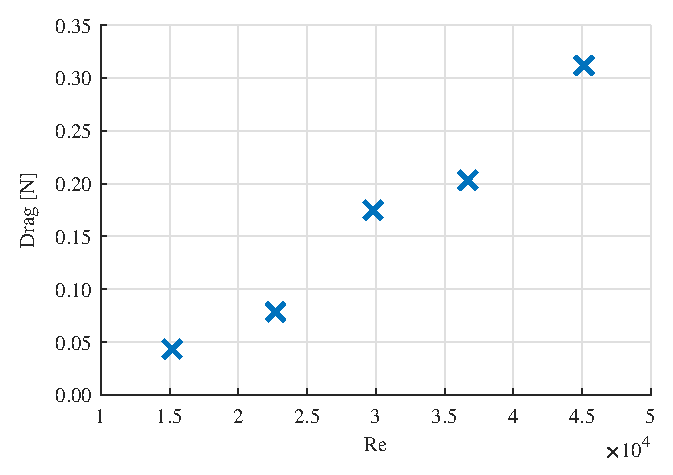
\includegraphics[width=\textwidth]{0_Images/SolidDragRe.eps}
        \caption{The drag.}
        \label{Fig:SolidDrag}
    \end{subfigure}
    ~
    \begin{subfigure}[b]{0.45\linewidth}
        \includegraphics[width=\textwidth]{0_Images/SolidCDRe.eps}
        \caption{The drag coefficient.}
        \label{Fig:SolidCD}
    \end{subfigure}
    \caption{Using the solid disk.}
    \label{fig:SolidDisk}
\end{figure}


\begin{figure} 
    \centering
    \begin{subfigure}[b]{0.45\linewidth}
        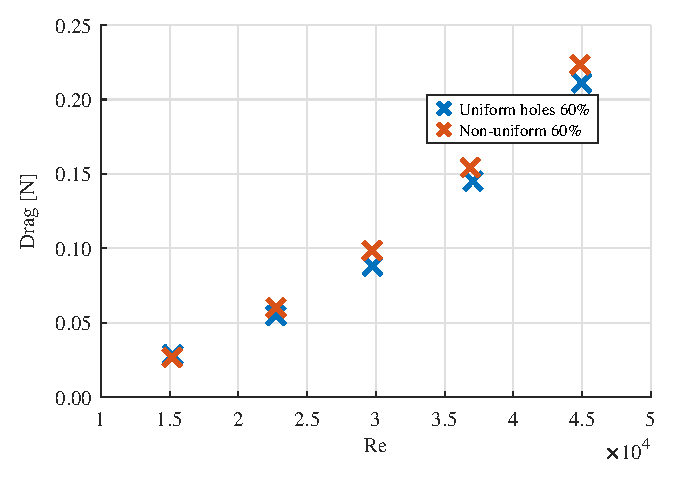
\includegraphics[width=\textwidth]{0_Images/SixtyDragRe.eps}
        \caption{The drag.}
        \label{Fig:SixtyDrag}
    \end{subfigure}
    ~
    \begin{subfigure}[b]{0.45\linewidth}
        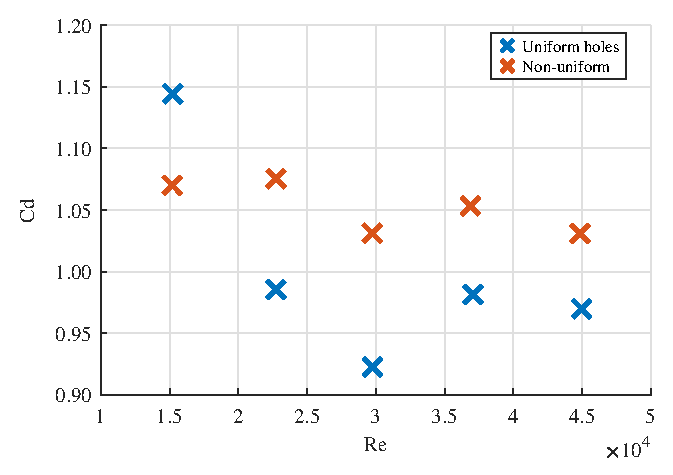
\includegraphics[width=\textwidth]{0_Images/SixtyCDRe.eps}
        \caption{The drag coefficient.}
        \label{Fig:SixtyCD}
    \end{subfigure}
    \caption{Using the disks with 60\% solidity.}
    \label{fig:SixtyDisk}
\end{figure}

\FloatBarrier

Further, the drag and drag coefficient for the disks with 40\% and 35\% solidity were plotted in figure \ref{fig:FortyDrag} and \ref{fig:FortyCD}, respectively. As these disks produced a drag fairly close to the average drag of the \gls{RWTM}s, the average drag and drag coefficient representing the rotating models is also included in the plots, to ease the comparison. 

%The average drag coefficient and standard deviation can be seen in table \ref{tab:AvgCD}. 

\begin{figure}
    \centering
    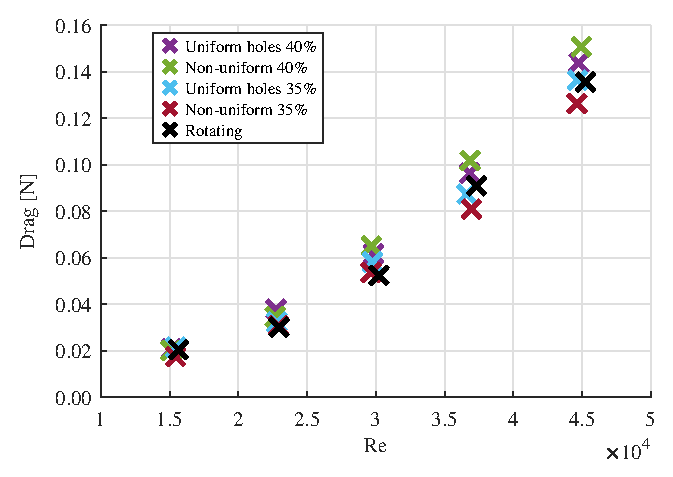
\includegraphics[width=0.8\linewidth]{0_Images/FortyDragRe.eps}
    \caption{The drag for the disks with 40\% and 35\% solidity, compared to the average drag coefficient of the rotating disks.}
    \label{fig:FortyDrag}
\end{figure}

\begin{figure}
    \centering
    \includegraphics[width=0.8\linewidth]{0_Images/FortyCDRe.eps}
    \caption{The drag coefficient for the disks with 40\% and 35\% solidity, compared to the average drag coefficient of the rotating disks.}
    \label{fig:FortyCD}
\end{figure}



Some general trends can be observed from these graphs. For all the \gls{AD} and the \gls{RWTM} measurements, the drag is seen to increase with increasing wind velocity, as one would expect. 

%It can also be seen that the \gls{spider} produces a slightly higher drag compared to the \gls{holes} with the same solidity for 60\% and 40\% solidity. The same trend can not be seen at 35\% solidity, where \gls{holes} seem to produce the largest drag. However, as mentioned, the \gls{holes} design with 35\% solidity was created in a slightly different way than those with 40\% and 60\% solidity, and they may not be exactly comparable. 

Another trend that can readily be seen, is that the drag coefficient decreases with decreasing solidity. This coincides with what has been found in the literature. Lignarolo et al (2016) \cite{Lignarolo2016} presented a comparison between different drag coefficients as a function of solidity, based on the results presented in six different papers. % According to this, a solidity of 60\% results in a Cd of around 0.9, a solidity of 40\% results in a Cd between 0.5 and 0.6, and a 35\% solidity results in a Cd between 0.4 and 0.5.
 Compared, the \gls{AD}s used in this study results in a slightly higher drag coefficient for all the solidities. This can for example be caused by differences in inflow conditions, such as inflow turbulence, or due to the models being placed in the boundary layer in this study, in contrast to most cases in literature where the hub is in the free stream flow. However, Lignarolo et al also concludes that the drag coefficient seems to be linearly decreasing with decreasing solidity, which is also the case with the results from the current measurements. 
%EFFECT OF WALLS! 

For all the different \gls{AD}s and for the \gls{RWTM}s, the drag coefficient corresponding to 5 \si{\m\per\s} is significantly higher than for the other velocities, while the drag coefficient related to the other four velocities generally seem to concentrate around some mean value. This may be because the disks are much more sensitive to ... However, this result will not have any significant impact on the future work, as the future work will focus around higher velocities than 5 \si{\m\per\s}. 

Looking at figure \ref{fig:FortyCD}, the \gls{spider} with 35\% solidity and the \gls{holes} with 35\% solidity seem to best match the drag of the rotating model. To study this further, the average drag coefficient over the four wind velocities where the measurements already seem to gather around some mean, is calculated, and presented in table \ref{tab:AvgCD}. Thus, the closest match seems to be the \gls{spider} with 35\% solidity, and the second closest match seems to be the \gls{holes} with 35\% solidity.


\begin{table}
    \centering
    \begin{tabular}{l c c r}
         Disk type & Average Cd \\
         \hline
         Rotating average & 0.570 \\
         %Solid & 1.515 \\
         %Uniform holes, 60\% & 0.965 \\
         %Non-uniform, 60\% & 1.048\\
         %Uniform holes, 40\% & 0.662 \\
         %Non-uniform, 40\% & 0.673 \\
         Uniform holes, 35\% & 0.604  \\
         Non-uniform, 35\% & 0.560 \\
    \end{tabular}
    \caption{Average Cd for the rotating model and the disks with 35\% solidity.}
    \label{tab:AvgCD}
\end{table}

%for last one, 0.5843 without drift 



%Which SD is relevant? I have the ones for each measurement... But maybe the ones for Cd also? 

%\section{Noise and other possible sources of error}

%\begin{figure}[h!]
%    \centering
%    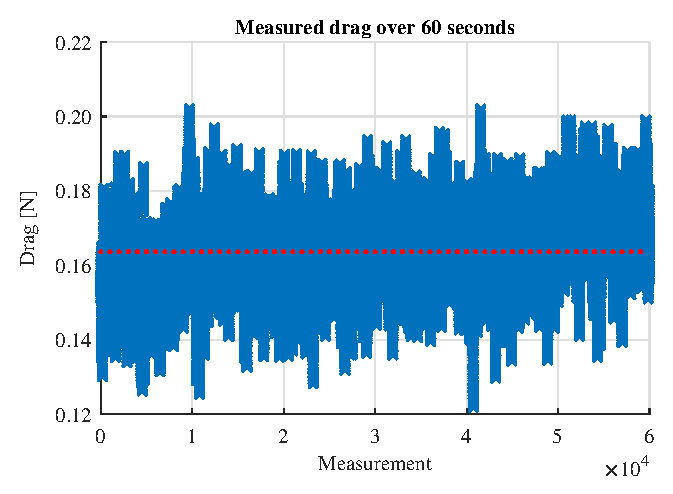
\includegraphics[width=\linewidth]{0_Images/NoiseFirst.eps}
%    \caption{The drag for the solid disk at 5 m/s.}
%    \label{fig:Noise}
%\end{figure}

%Figure \ref{fig:Noise} shows each measured drag value at a sampling rate of 1000 Hz over the course of 60 seconds. The measured drag varies with a 0.012, compared to an average of 0.1636. This means that the noise is of one order less that the average. 

%This noise may both be related to measurement noise in the force plate, and electrical noise as the signal passes from the force plate, through the amplifier and the lowpass filter. 
%It is still a reasonable assumption that the measurements have a Gaussian distribution and that the average drag is representative. 

Three additional remarks can be made related to the measurements. There does not seem to be any clear trends regarding the drag coefficient when using the \gls{spider} design compared to when using the \gls{holes} design. The measured temperature only varies between about 20\degree C and 23\degree C. Since this variation is fairly small, it is assumed to not have any significant impact on the resulting drag. Also, when studying the standard deviation for each 60 \si{\s} measurement, the standard deviation is always between 0.011 and 0.015, showing that this might be the size of the measurement noise related to the transducer and the electrical noise as the signal passes from the force plate, through the amplifier and the lowpass filter. 


\FloatBarrier
 


%Error, standard deviation 

%why do we get the results that we get? 

%- Adjusting for drift 
%- statistikk arument 
%- usikkerhet



